\documentclass[11pt]{article}

\usepackage[headings]{fullpage}
\usepackage{graphicx,amsmath}
\pagestyle{myheadings}
\markboth{Noise}{Noise}

\usepackage{amsmath}
\usepackage{bm}

\newcommand{\nat}{\mathbb{N}}          % Natural numbers
\newcommand{\integer}{\mathbb{Z}}      % Integers
\newcommand{\real}{ {\mathbb{R}} }     % Reals
\newcommand{\float}{ {\mathbb{F}} }     % Reals
\newcommand{\rmn}[2]{ \mathbb{R}^{#1\times#2} }     % Reals
\newcommand{\complex}{ {\mathbb{C}} }  % Complex
\newcommand{\macheps}{\ensuremath \varepsilon_{\text{mach}}}

\renewcommand{\Re}{\operatorname{Re}}
\renewcommand{\Im}{\operatorname{Im}}

% Boldface vectors
\newcommand{\bff}{\bm{f}}
\newcommand{\bfF}{\bm{F}}
\newcommand{\bfw}{\bm{w}}
\newcommand{\bfv}{\bm{v}}
\newcommand{\bfe}{\bm{e}}
\newcommand{\bfc}{\bm{c}}
\newcommand{\bfp}{\bm{p}}
\newcommand{\bfq}{\bm{q}}
\newcommand{\bfr}{\bm{r}}
\newcommand{\bfs}{\bm{s}}
\newcommand{\bfu}{\bm{u}}
\newcommand{\bfb}{\bm{b}}
\newcommand{\bfx}{\bm{x}}
\newcommand{\bfy}{\bm{y}}
\newcommand{\bfg}{\bm{g}}
\newcommand{\bfh}{\bm{h}}
\newcommand{\bfz}{\bm{z}}
\newcommand{\bfa}{\bm{a}}
\newcommand{\bft}{\bm{t}}
\newcommand{\bfd}{\bm{d}}
\newcommand{\bfalpha}{\bm{\alpha}}
\newcommand{\bfeps}{\bm{\varepsilon}}
\newcommand{\bfdelta}{\bm{\delta}}
\newcommand{\bfzero}{\bm{0}}
\newcommand{\eye}[1]{\bfe_{#1}}

% Boldface matrix
\newcommand{\m}[1]{\bm{#1}}
\newcommand{\mA}{\m{A}}
\newcommand{\mL}{\m{L}}
\newcommand{\mF}{\m{F}}
\newcommand{\mU}{\m{U}}
\newcommand{\mJ}{\m{J}}
\newcommand{\mP}{\m{P}}
\newcommand{\mQ}{\m{Q}}
\newcommand{\mR}{\m{R}}
\newcommand{\mD}{\m{D}}
\newcommand{\mS}{\m{S}}
\newcommand{\mB}{\m{B}}
\newcommand{\mC}{\m{C}}
\newcommand{\mE}{\m{E}}
\newcommand{\mG}{\m{G}}
\newcommand{\mH}{\m{H}}
\newcommand{\mV}{\m{V}}
\newcommand{\mW}{\m{W}}
\newcommand{\mX}{\m{X}}
\newcommand{\mZ}{\m{Z}}
\newcommand{\mK}{\m{K}}
\newcommand{\mM}{\m{M}}

\newcommand{\meye}{\m{I}}

\newcommand{\ee}[1]{\times 10^{#1}}
\newcommand{\jac}[2]{\frac{\bfd \bm{#1}}{\bfd \bm{#2}}}
\newcommand{\diag}{\operatorname{diag}}
\newcommand{\fl}{\operatorname{fl}}
\newcommand{\circop}[1]{\makebox[0pt][l]{$\bigcirc$}\hspace{1pt}#1}
\newcommand{\myvec}{\operatorname{vec}}
\newcommand{\unvec}{\operatorname{unvec}}
\newcommand{\kron}[2]{#1 \otimes #2}


\begin{document}

\begin{center}
  \bf Project: That's one thing he hated! The
  NOISE! NOISE! NOISE! NOISE!   
\end{center}

Most digital images are captured by a photoelectric sensor array. If
the array is divided into many small pixels, then the number of
photons gathered by each pixel may be small, and random fluctuations
can cause ``noise'' in the image. For our purposes we model noise by
the addition at each image array element of a normally distributed
random number with average zero. Hence for an $n\times n$ image,
\begin{verbatim}
Z = X + sigma*randn(n)/n;
\end{verbatim}

There is no perfect way to remove noise once it has been added. One
solution is to apply a good dose of blurring, but this tends to remove
features of interest as well as noise. Instead there is a method
called constrained least squares inverse filtering. In this model we
have to assume knowledge about the strength $\sigma$ of noise
added. If we write the noisy image $\mZ$ as a vector $\bfz$, we can
describe the result of the process as the $\bfu$ satisfying
\begin{equation}
  \label{min}
  \min \| \mR\bfu \|, \quad \text{subject to} \quad \| \bfu - \bfz \| = \sigma.
\end{equation}
Here $\mR$ is a ``roughing'' operator. It is meant to exaggerate and
thus penalize discontinuities. As is often the case, we find it
convenient to describe and compute the action of $\mR$ on the matrix
form $\mV$ of an image vector $\bfv$:
\begin{equation}
  \label{rough}
  \mR\bfv \leftrightarrow \mD\mV + \mV\mD,
\end{equation}
where $\mD$ is the matrix
\begin{equation}
  \mD = 
  \begin{bmatrix}
    -2 & 1 & & \\
    1 & -2 & 1 & \\
    & \ddots & \ddots & \ddots \\
    & & 1 & -2
  \end{bmatrix}.
\end{equation}
In words, \eqref{min} says the solution to the problem is the least rough
image $\bfu$ that is the same distance from the noisy image as the
original.

As a constrained minimization, equation~\eqref{min} has a solution in terms of
a Lagrange multiplier $\gamma>0$. After some work, the solution is
\begin{equation}
  \label{sol}
  \bfu = (\meye + \gamma \mR^2 )^{-1} \bfz,
\end{equation}
where $\gamma$ is chosen so that 
\begin{equation}
  \label{root}
  f(\gamma) = \|\bfu-\bfz\|^2 - \sigma^2 = 0.
\end{equation}
This is a rootfinding problem for $\gamma$. Note that each evaluation
of $f$ requires the solution of a linear system of equations for $\bfu$.
This system is large and will be solved using GMRES. However, you
don't have the matrix $\mR$, so you will have to use GMRES in its
matrix-free mode. (Make sure you monitor the GMRES flag output
so that returned values are really solutions.)



\textbf{To make this project simpler, choose $\mX$ to be a \emph{square}
  image of size no larger than $250\times 250$.} If you use a
photograph, start with a high-res image and crop to the smaller size
to get a good image. Also use an image with a good combination of dark
and light pixels, rather than mostly black or mostly white.

\begin{figure}[htbp]
  \centering
  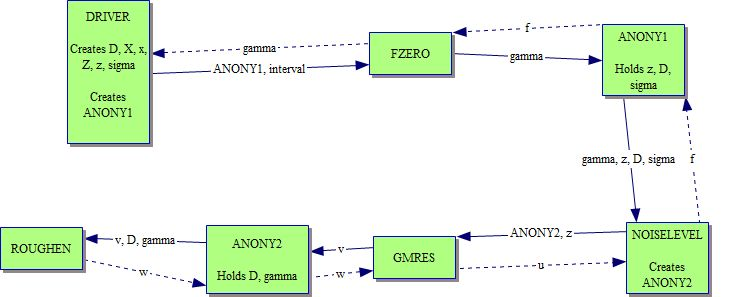
\includegraphics[width=6.5in]{codestruct}  
\end{figure}
The structure of the code you need for this problem is shown in the
figure. You need to write 
\begin{itemize}
\item Function \texttt{roughen}, which returns $\bfw=(\meye+\gamma \mR^2)\bfv = \bfv
  + \gamma \mR^2\bfv$ for any given vector $\bfv$. This includes some
  reshaping, and applying~\eqref{rough} two times.
\item Function \texttt{noiselevel}, which calculates $f$ in
  equation~\eqref{root} above after GMRES has been called to find $\bfu$.
\item A top-level driver that defines the images, the value of
  \texttt{sigma}, and the matrix $\mD$ needed by \texttt{roughen}. Once
  \texttt{fzero} has found the correct value of $\gamma$, you need to
  call GMRES one more time to find the $\bfu$ from~\eqref{sol}. The result is the
  method's optimal reconstruction of $\bfx$, which is reshaped to find $\mX$.
\end{itemize}
There are also two ``wrapper'' anonymous functions needed to pass
extra values through \texttt{fzero} and \texttt{gmres}. These are
one-liners like in the earlier project and the homework.

Your goal is to apply noise with \texttt{sigma} equal to $8n$, $16n$,
and $32n$, and then apply reconstruction in each case. Report your
$\gamma$ solution each time (it should increase with $\sigma$ and stay
less than or at least close to 1), and show the noisy and
reconstructed images side by side each time.


\end{document}
